\newpage
\chapter{MIDAS}
\label{chap:mc}
\workTodo{In diesem Kapitel werden grundlegende Themen behandelt, die im Rahmen des Forschungsprojekts zum Verst�ndnis der Ausrei�er-Erkennung in Graphen gedient haben.}

Erst erkl�ren wie der MIDAS funktioniert. Und zum Laufen gebracht mit Graphen �ber die Zeit ENRON \& DARPA. Im Anschluss auf Zeitreihendaten angewendet.

\section{Grundlagen}
\label{sec:mc-gl}
\workTodo{Einf�hrung in den Algorithmus}


\subsection{Count-min Sketch}
\label{sec:mc-gl-cms}

\subsubsection{Einf�hrung}
\label{sec:mc-gl-cms-in}

\workTodo{Stichworte sammeln}

\section{Ergebnisse Ausrei�ererkennung in Zeitreihen}
Wie in \autoref{chap:trsnsMidas} beschrieben muss die Zeitreihe zun�chst in verschiedene Netzwerke umgewandelt werden. In \autoref{img:midasTSresults} ist das Ergebnis der Ausrei�ererkennung mit Midas abgebildet. Der Ausrei�er wird von dem Algorithmus identifiziert, jedoch ist der Verlauf des Ausrei�er Scores schwierig zu interpretieren. Es ist zu erkennen, das zu beginn jedes Abschnittes der Ausrei�er Score sehr hoch ist und am Ende niedrig(Ausnahme Abschnitt mit Ausrei�er). Grund hierf�r ist, das der Algorithmus die Anzahl der Kanten in einem Abschnitt mit der Anzahl an Katen aus vorherigen Abschnitten vergleicht. Zu Beginn eines jeden Abschnitts ist die Anzahl an Kanten deutlich geringer, deshalb ist der Ausrei�er Score auch h�her. Am Ende eines Abschnitts ist die Anzahl an Kanten in Relation identisch, deshalb ist der Ausrei�er Score h�her. Der Abschnitt in welchem sich der Ausrei�er befindet ist deutlich gr��er als die anderen Abschnitte. Der Grund hierf�r ist, das die Anzahl an Kanten deutlich h�her ist als in den anderen Abschnitten. F�r jede Kante wird ein zus�tzliches Element zum Ausrei�er Score hinzugef�gt. Da Kantengewichte in dem Abschnitt mit dem Ausrei�er deutlich gr��er sind, resultiert dies in deutlich mehr Kanten. 
\label{sec:resultsOTs}

\begin{figure}[h]
	\centering
	\subfloat[Caption for sub-figure1]{
		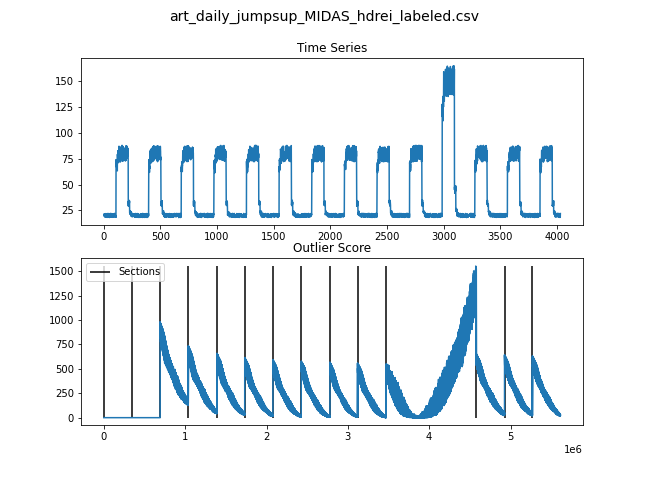
\includegraphics[width=0.5\textwidth]{fig/resultsMidasTS/art_daily_jumpsup_MIDAS_hdrei_labeled_result.png}}
	\label{img:midasTSresult}
	\subfloat[Caption for sub-figure1]{
		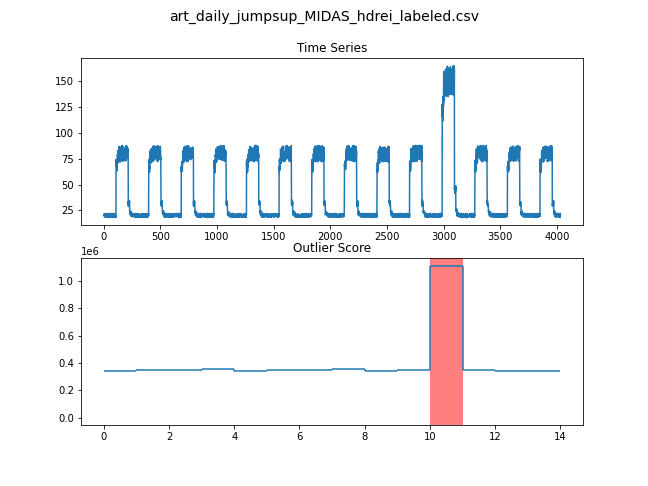
\includegraphics[width=0.5\textwidth]{fig/resultsMidasTS/result_without_midas.png}}
	\label{img:reultwoMidas}
	\caption{Vergelich Perculation Algorithmus mit Sliding Window Verfahren und ohne Sliding Window Verfahren}
	\label{img:midasTSresults}
\end{figure}

Da der Midas Algorithmus lediglich die Anzahl an Kanten zwischen zwei Knoten z�hlt um Ausrei�er zu erkennen, verglichen wir den Midas Algorithmus mit einem naiven Algorithmus der lediglich die Gesamtanzahl an Knoten in einem Abschnitt z�hlt. Es konnte festgestellt werden, dass der naive Ansatz den Midas Algorithmus mithalten kann. Aus diesem Grund wurden keinerlei weitere Datens�tze untersucht. 
\workTodo{Vielleicht den Algorithmus einmal auf einzelne Peaks testen vielleicht bringt das was.}
\label{sec:resultTSwithoutMidas}

